\documentclass[tikz]{standalone}
%\usetikzlibrary{...}% tikz package already loaded by 'tikz' option
\usepackage{amsmath,amssymb}  % Pour les symboles mathématiques
\usepackage{lmodern}          % Utilisation de la police lmodern pour meilleure compatibilité SVG
\usetikzlibrary{matrix,positioning}
\usetikzlibrary{arrows.meta}
\usetikzlibrary{calc}
\begin{document}

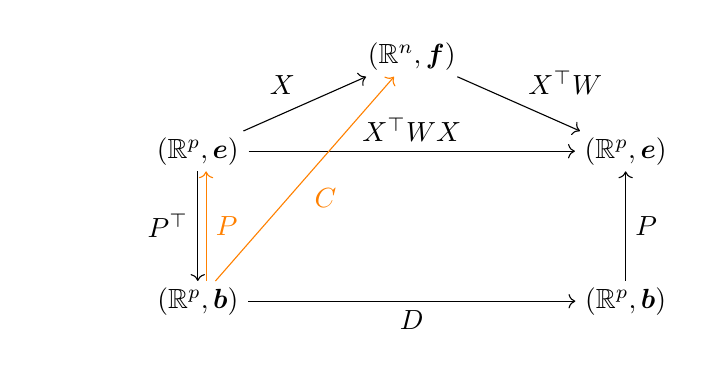
\begin{tikzpicture}
  \matrix (m) [matrix of math nodes, row sep=2em, column sep=4em, text height=1.5ex, text depth=0.25ex]
  {
  	&  & (\mathbb{R}^n, \boldsymbol{f}) & \\
    & (\mathbb{R}^p, \boldsymbol{e})  & &(\mathbb{R}^p, \boldsymbol{e}) \\
    & & &\\
    & (\mathbb{R}^p, \boldsymbol{b}) & &(\mathbb{R}^p, \boldsymbol{b}) \\
  };

  % Flèches entre les cellules
  \path[->] (m-2-2) edge node[above] {$X^\top W X$} (m-2-4);
  \path[->] (m-2-2) edge node[left] {$P^\top$} (m-4-2);
  \path[->] (m-4-4) edge node[right] {$P$} (m-2-4);
  \path[->] (m-4-2) edge node[below] {$D$} (m-4-4);  
  \path[->] (m-2-2) edge node[above left] {$X$} (m-1-3);
  \path[->] (m-1-3) edge node[above right] {$X^\top W$} (m-2-4);
  \path[->, color=orange] (m-4-2) edge node[below right] {$C$} (m-1-3);
  \path[->, color=orange] ([xshift=3pt]m-4-2.north) edge node[right] {$P$} ([xshift=3pt]m-2-2.south);
   
\end{tikzpicture}

\end{document}